\chapter{Implementation}\label{ch:Implementation}

\section{Exploratory Data Analysis}
All code for the EDA detailed in this chapter can be found at:\newline https://github.com/AMacleod79/HonoursProjectCode
\subsection{Data Overview}
\subsubsection{Cervical cancer dataset}
The cervical cancer dataset was obtained from kaggle.com. \newline
(see https://www.kaggle.com/loveall/cervical-cancer-risk-classification)\newline
This dataset does not look at predicting if someone will or will not have cervical cancer, however it looks at attributing a risk factor for cervical cancer or not. Cervical cancer is a complicated diagnostic to make and as such there is not one single test to confirm diagnostic. The positive risk factor is inferred from the combination of the last four column: Hinselmann, Schiller, Citology, Biopsy \cite{Fernandes:2017td} (also cite the discussion page on kaggle).
The dataset contains 858 instances with 32 features and 4 target variables for each of the test carried out.
The exploratory data analysis carried out on this dataset can be found in the cited github repository as CervicalCancerEDA.R.
The 32 features focus on lifestyle factors previously shown to influence cervical cancer risk in women, namely:
%need to list the attributes here
An examination of the data structure showed that 27 columns were factors, with the column "smoke pack per year" showing 63 levels. The Random Forest function in R will only handle a maximum of 53 levels and therefore the data in this column needed to be manipulated to accommodate this restriction. First any missing values was replaced by the mean for the column. Then it was found that there were a high number of discrete values between 0 and 1 for the number of pack of cigarettes smoked per year, and these were all considered as independent levels. All values that were less than 1 for this column were replaced by 0, taking the total number of levels for the column from 63 to 42, which is now manageable by Random Forest.
All the other columns had a number of factor levels smaller than 53 and were left as such, however any missing value was replaced by the mean for the column in which it was found.
A composite target variable calculated as a mean value of all 4 target variables (Hinselmann, Schiller, Citology, Biopsy was created and added as the last column in the dataset (rounded to 0 or 1).
Finally the class distribution was represented as a bar chart (see Figure 4.1) and the modified dataset was exported as a new csv file to be used in the later stages of this projects.

\begin{figure}[H]
    \centering
    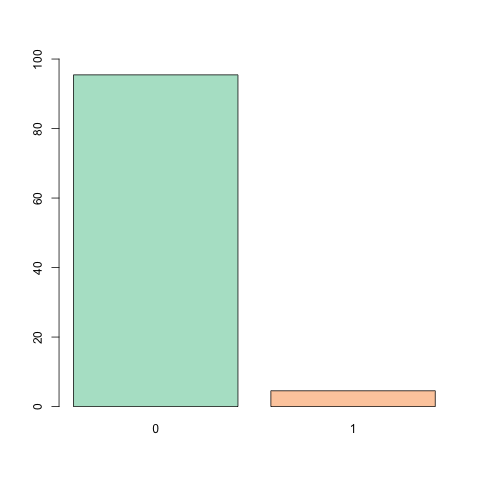
\includegraphics[width=0.8\textwidth]{ThesisTemplate/usingLatex/chapter4Images/figure4_10.png}
    \caption{Class Distribution of cervical cancer dataset.\newline
    0 represents the absence of cervical cancer risk for an individual and 1 represent the presence of cervical cancer risk.}
    \label{fig:my_label}
\end{figure}


\subsubsection{Breast cancer dataset}
This dataset was obtained from kaggle.com. \newline
(see https://www.kaggle.com/uciml/breast-cancer-wisconsin-data) \newline
This dataset was developed with a view to train and test algorithms to determine whether a breast tumour was malignant or benign \cite{}. \newline
% need citation here
The dataset is comprised of 569 instances each with 32 attribute and one target label (B for benign and m for malignant).\newline
The attributes were computed from images of a fine needdle aspirate of a breast mass to describe the characteristics of the cell nuclei present in the image. The features were as follows:
\begin{itemize}
    \item radius (mean of distances from center to points on the perimeter)
    \item texture (standard deviation of gray-scale values) 
    \item perimeter 
    \item area 
    \item smoothness (local variation in radius lengths) 
    \item compactness (perimeter\^2 / area - 1.0)
    \item concavity (severity of concave portions of the contour)
    \item concave points (number of concave portions of the contour)
    \item symmetry
    \item fractal dimension ("coastline approximation" - 1)
\end{itemize}
The mean, standard error and mean of of three largest values (i.e. the "worst") for each of the feature was calculated and documented as a feature for each image.\newline

The exploratory data analysis carried out on this dataset is documented in the cited github repository as BreastCancerEDA.R.\newline
An analysis of the data structure showed no missing values. The target variable was expressed as B or M and was recoded to be either 0 (begign) or 1 (malignant), further the target variable was originally the second column but for ease of analysis in the next stages of the project this was moved to be the last column and renamed "Label".
Finally the class distribution of the dataset was computed and is shown in figure 4.2 and the modified dataset was exported as a csv file for later use in the project.

\begin{figure}[H]
    \centering
    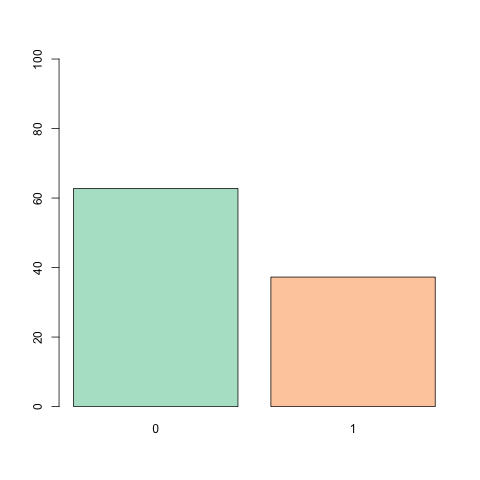
\includegraphics[width=0.8\textwidth]{ThesisTemplate/usingLatex/chapter4Images/figure4_4.png}
    \caption{Class Distribution of the breast cancer dataset.\newline 0 represents the cases were the breast mass was benign and 1 those cases were the mass was malignant.}
    \label{fig:my_label}
\end{figure}

\subsubsection{Liver Disease dataset}

This dataset was obtained from kaggle.com.\newline
(see https://www.kaggle.com/jeevannagaraj/indian-liver-patient-dataset). \newline
%citation needed here
This dataset is made up of 583 instances of patient records with 10 attributes and one target variable to determine whether the patient is a liver patient or not. The attributes are various biochemical measures of liver health as well as patient specific information such as age and gender:
\begin{itemize}
    \item Age of patient
    \item Gender of patient
    \item Total Bilirubin
    \item Direct Bilirubin
    \item Alkaline Phosphatase
    \item Alamine Amino-transferase (sgpt)
    \item Aspartate Amino-transferase (sgot)
    \item Total Proteins
    \item Albumin
    \item Albumin and Globulin Ratio
    \item is patient (target label)
\end{itemize}

The exploratory data analysis carried out on this dataset is documented in the cited github repository as LiverDataEDA.R.\newline
The target label was set to 1 (not a liver patient) and 2 (liver patient), for consistency with respect to the other dataset used in this project, the data was recoded to 0 (not a liver patient) and 1 (liver patient).\newline
A check for missing data revealed only four instances missing a value in the albumin and globulin ratio. The missing values were replaced with the mean for that column.
The class distribution was compiled and presented as a graph (see figure 4.3) and the modified dataset was exported as a csv file for later use in the project.

\begin{figure}[H]
    \centering
    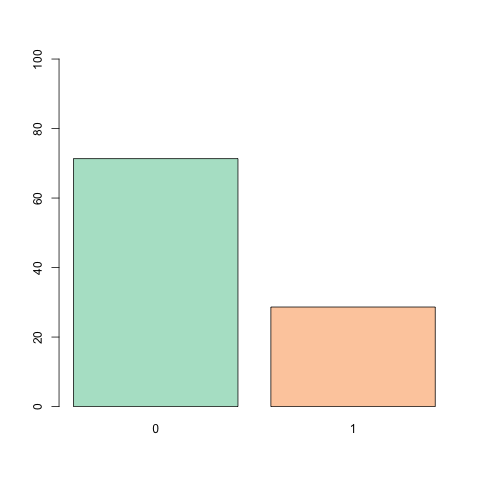
\includegraphics[width=0.8\textwidth]{ThesisTemplate/usingLatex/chapter4Images/figure4_6.png}
    \caption{Class Distribution of the liver dataset.\newline 0 represents the cases were the patient was not identified as a liver patient and 1 represents those cases were the patient was identified as a liver patient.}
    \label{fig:my_label}
\end{figure}

\subsubsection{Diabetes}
This dataset comprise 768 instances of health data from female Pima Indian patients of at least 21 years of age. There are 8 attributes and one target variable. The target variable indicates whether the individual will develop diabetes within 5 years (1) or not (0). The attributes were as follows:
\begin{itemize}
    \item Pregnancies indicates the number of times the patient pregnant
    \item GlucosePlasma indicates the glucose concentration at 2 hours in an oral glucose tolerance test
    \item BloodPressureDiastolic indicates the diastolic blood pressure (mm Hg)
    \item SkinThicknessTriceps indicates triceps skin fold thickness ( in mm)
    \item Insulin2-Hour indicates the serum insulin concentration  (mu U/ml)
    \item BMI indicates body mass index (weight in kg/(height in m \textsuperscript{2})
    \item DiabetesPedigreeFunctionDiabetes is a pedigree function calculated by the original authors of the study which takes family history of diabeted into account
    \item Age records the age of the patient (years)
\end{itemize}
 The dataset was used in a study looking at the ADAP algorithm and further details about the pedigree function and other variables can be found in the article \cite{Smith:1988wy}.
 
The exploratory data analysis carried out on this dataset is documented in the cited github repository as DiabetesEDA.R.\newline
The target label was already set to 0 (did not develop diabetes within 5 years) and 1 (did develop diabetes within 5 years), so no recoding of the data was necessary.\newline
A check for missing data revealed none, and Smith \textit{et al.,} indicate that they replaced any missing data with 0 (which does not always make sense, e.g. for blood pressure). No further modification of the dataset were necessary and the dataset was saved as csv file for later use.
The class distribution was compiled and presented as a graph (see figure 4.4).

\begin{figure}[H]
    \centering
    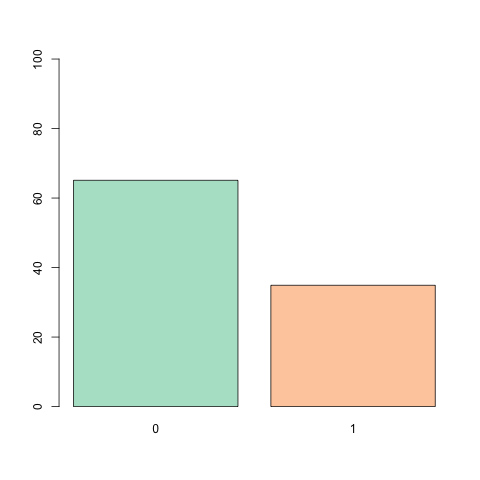
\includegraphics[width=0.8\textwidth]{ThesisTemplate/usingLatex/chapter4Images/figure4_8.png}
    \caption{Class Distribution of the diabetes dataset.\newline 0 represents the cases were the patient did not develop diabetes within 5 years and 1 represents the cases where the patient did develop diabetes within 5 years.}
    \label{fig:my_label}
\end{figure}

\subsubsection{Lower Back Pain dataset}
\subsubsection{Heart Attack Dataset}
\subsubsection{Autism dataset}
\subsubsection{Fertility dataset}

\subsection{Class distribution}


\begin{table}[H]
\centering
\begin{tabular}{lrl}
  \hline
Dataset & Percentage & Category \\ 
  \hline
Cervical\_Cancer & 95.45 & Majority Class \\ 
  Cervical\_Cancer & 4.55 & Minority Class \\ 
  Breast\_Cancer & 62.74 & Majority Class \\ 
  Breast\_Cancer & 37.26 & Minority Class \\ 
  Liver\_Disease & 71.36 & Majority Class \\ 
  Liver\_Disease & 28.64 & Minority Class \\ 
  Diabetes & 65.10 & Majority Class \\ 
  Diabetes & 34.90 & Minority Class \\ 
  Lower\_Back\_Pain & 32.26 & Majority Class \\ 
  Lower\_Back\_Pain & 67.74 & Minority Class \\ 
  Lower\_Back\_Pain(modified) & 87.72 & Majority Class \\ 
  Lower\_Back\_Pain(modified) & 12.28 & Minority Class \\ 
  Heart\_Attack & 63.95 & Majority Class \\ 
  Heart\_Attack & 36.05 & Minority Class \\ 
  Heart\_Attack(modified) & 94.95 & Majority Class \\ 
  Heart\_Attack(modified) & 5.05 & Minority Class \\ 
  Autism & 73.15 & Majority Class \\ 
  Autism & 26.85 & Minority Class \\ 
  Fertility & 88.00 & Majority Class \\ 
  Fertility & 12.00 & Minority Class \\ 
   \hline
\end{tabular}
\end{table}

\begin{figure}[H]
    \centering
    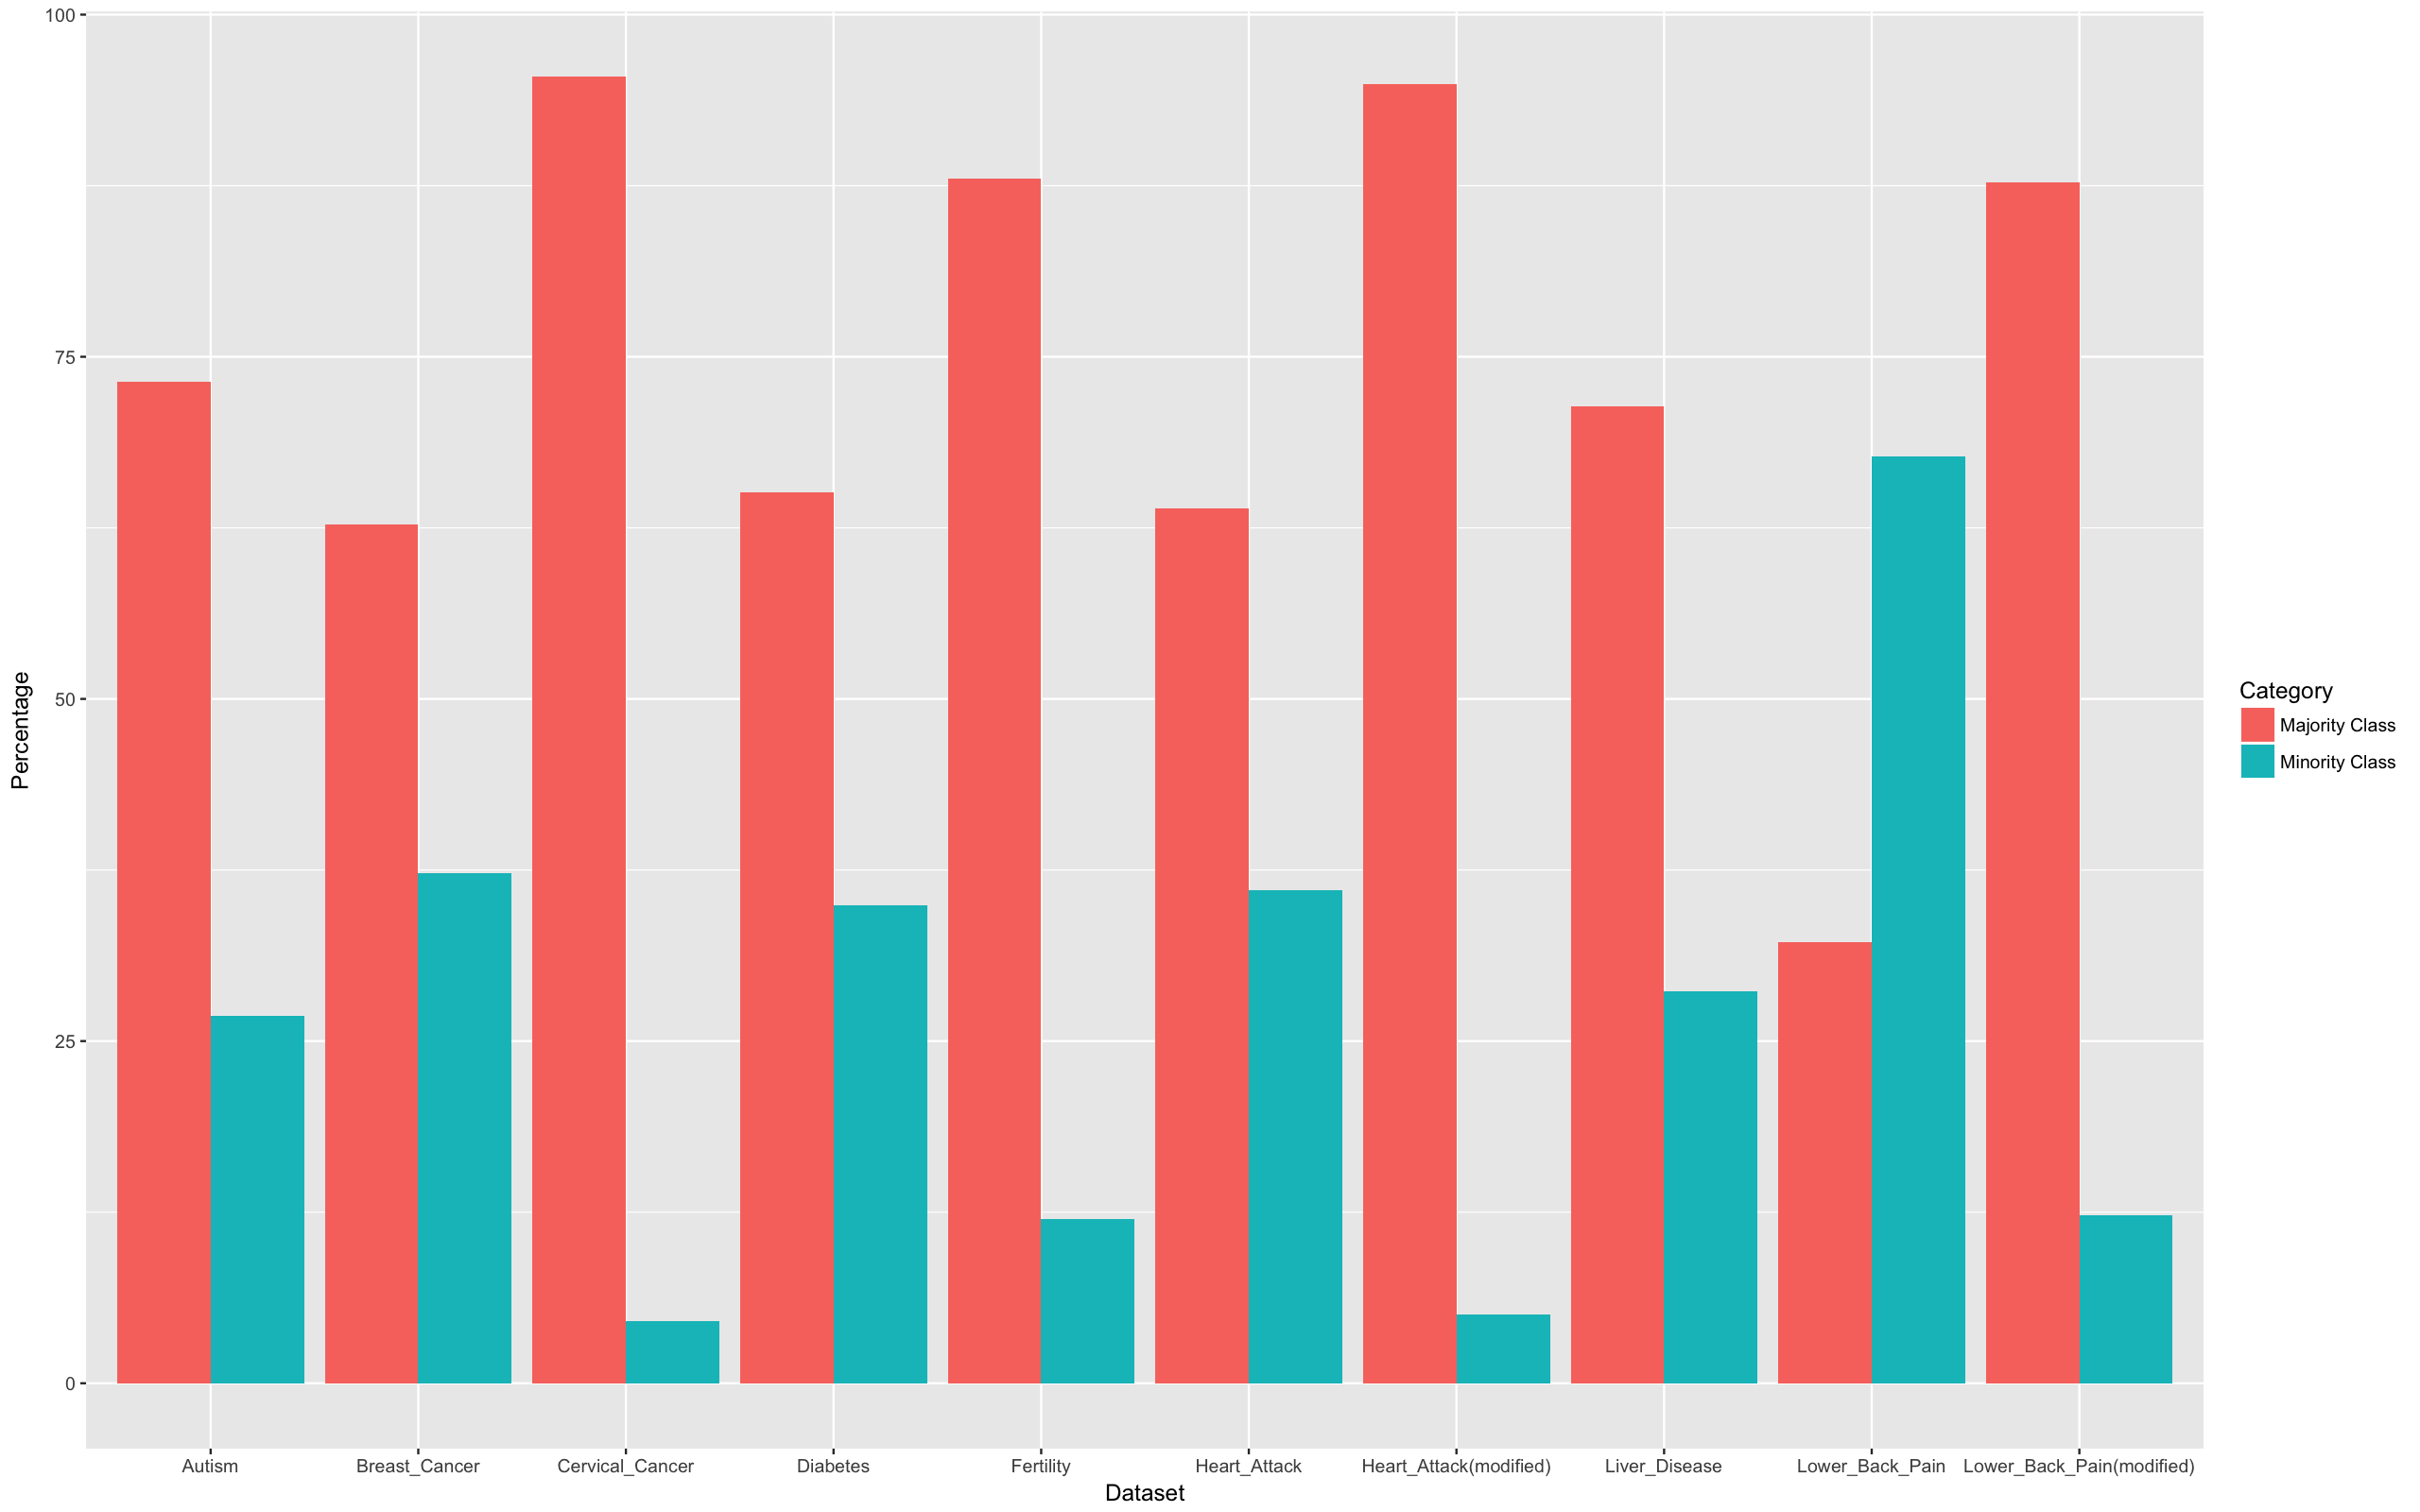
\includegraphics[width=0.8\textwidth]{ThesisTemplate/usingLatex/chapter4Images/figure4_1b.png}
    \caption{Class Distribution of the chosen datasets.\newline In all cases the majority class is the class representing healthy subjects and the minority class is the class representing affected subjects. In the case of the lower back pain dataset, the class representing the "abnormal" patients counts more instances than the the class representing the "normal" patients, however the terms minority and majority were kept for consistency with the other datasets.}
    \label{fig:my_label}
\end{figure}
\section{Modelling the datasets}
\subsection{Random Forest}
\begin{table}[ht]
\centering
\begin{tabular}{lrrrr}
  \hline
Dataset & Accuracy & Sensitivity & Precision & F1Score \\ 
  \hline
AuSDf & 100.00 & 1.00 & 1.00 & 1.00 \\ 
  BCDf & 91.67 & 0.86 & 0.94 & 0.89 \\ 
  CCDf & 93.75 & 0.33 & 0.45 & 0.38 \\ 
  DiabetesDf & 74.12 & 0.56 & 0.72 & 0.63 \\ 
  FertDf & 93.10 & 0.00 &  &  \\ 
  HAPDf & 90.80 & 0.83 & 0.89 & 0.86 \\ 
  LBPDf & 81.52 & 0.90 & 0.84 & 0.87 \\ 
  LiverDf & 71.68 & 0.35 & 0.58 & 0.44 \\ 
   \hline
\end{tabular}
\end{table}
\subsection{Support Machine Vector}
\subsection{K-Nearest Neighbour}
\subsection{Naive  Bayes}
\section{Modelling the datasets with data-level solutions applied}
\subsection{Undersampling of the majority class}
undersampling majority class 40\%
\begin{table}[ht]
\centering
\begin{tabular}{lrrrr}
  \hline
Dataset & Accuracy & Sensitivity & Precision & F1Score \\ 
  \hline
AuSDf & 100.00 & 1.00 & 1.00 & 1.00 \\ 
  BCDf & 94.23 & 0.98 & 0.93 & 0.96 \\ 
  CCDf & 95.45 & 0.75 & 0.82 & 0.78 \\ 
  DiabetesDf & 69.06 & 0.88 & 0.62 & 0.73 \\ 
  FertDf & 92.31 & 0.67 & 1.00 & 0.80 \\ 
  HAPDf & 81.13 & 0.90 & 0.80 & 0.85 \\ 
  LBPDf & 93.06 & 1.00 & 0.92 & 0.96 \\ 
  LiverDf & 70.71 & 0.86 & 0.62 & 0.72 \\ 
   \hline
\end{tabular}
\end{table}

undersampling majority class 60\%
\begin{table}[ht]
\centering
\begin{tabular}{lrrrr}
  \hline
Dataset & Accuracy & Sensitivity & Precision & F1Score \\ 
  \hline
AuSDf & 100.00 & 1.00 & 1.00 & 1.00 \\ 
  BCDf & 96.03 & 0.94 & 0.98 & 0.96 \\ 
  CCDf & 92.50 & 0.61 & 0.69 & 0.65 \\ 
  DiabetesDf & 70.24 & 0.78 & 0.65 & 0.71 \\ 
  FertDf & 77.78 & 0.00 & 0.00 &  \\ 
  HAPDf & 79.69 & 0.69 & 0.92 & 0.79 \\ 
  LBPDf & 78.75 & 0.92 & 0.82 & 0.86 \\ 
  LiverDf & 64.75 & 0.46 & 0.54 & 0.49 \\ 
   \hline
\end{tabular}
\end{table}

undersampling majority class 75\%
\begin{table}[ht]
\centering
\begin{tabular}{lrrrr}
  \hline
Dataset & Accuracy & Sensitivity & Precision & F1Score \\ 
  \hline
AuSDf & 100.00 & 1.00 & 1.00 & 1.00 \\ 
  BCDf & 95.10 & 0.90 & 1.00 & 0.95 \\ 
  CCDf & 95.38 & 0.74 & 0.78 & 0.76 \\ 
  DiabetesDf & 75.26 & 0.64 & 0.70 & 0.67 \\ 
  FertDf & 85.71 & 0.50 & 0.33 & 0.40 \\ 
  HAPDf & 83.33 & 0.75 & 0.81 & 0.78 \\ 
  LBPDf & 86.90 & 0.94 & 0.90 & 0.92 \\ 
  LiverDf & 61.70 & 0.31 & 0.52 & 0.39 \\ 
   \hline
\end{tabular}
\end{table}


\subsection{Oversampling of the minority class}
Oversampling using SMOTE (retain majority class, oversample 100\%)
100, 400
table showing training set distribution before and after smote
\begin{table}[ht]
\centering
\begin{tabular}{lrrrr}
  \hline
Dataset & MajorityClass & MinorityClass & NewMajorityClass & NewMinorityClass \\ 
  \hline
AuSDf & 353 & 140 & 560 & 280 \\ 
  BCDf & 258 & 143 & 572 & 286 \\ 
  CCDf & 573 &  29 & 116 &  58 \\ 
  DiabetesDf & 362 & 178 & 712 & 356 \\ 
  FertDf &  61 &  10 &  40 &  20 \\ 
  HAPDf & 131 &  76 & 304 & 152 \\ 
  LBPDf &  71 & 147 & 142 & 284 \\ 
  LiverDf & 297 & 113 & 452 & 226 \\ 
  subHAPDf & 134 &   7 &  28 &  14 \\ 
  subLBPDf &  74 &   8 &  32 &  16 \\ 
   \hline
\end{tabular}
\end{table}


\begin{table}[ht]
\centering
\begin{tabular}{lrrrr}
  \hline
Dataset & Accuracy & Sensitivity & Precision & F1Score \\ 
  \hline
AuSDf & 100.00 & 1.00 & 1.00 & 1.00 \\ 
  BCDf & 93.45 & 0.90 & 0.94 & 0.92 \\ 
  CCDf & 97.66 & 0.90 & 0.64 & 0.75 \\ 
  DiabetesDf & 75.00 & 0.62 & 0.71 & 0.66 \\ 
  FertDf & 75.86 & 0.50 & 0.14 & 0.22 \\ 
  HAPDf & 88.51 & 0.83 & 0.83 & 0.83 \\ 
  LBPDf & 78.26 & 0.84 & 0.84 & 0.84 \\ 
  LiverDf & 71.10 & 0.56 & 0.54 & 0.55 \\ 
  subHAPDf & 92.98 & 0.33 & 0.33 & 0.33 \\ 
  subLBPDf & 93.75 & 0.67 & 1.00 & 0.80 \\ 
   \hline
\end{tabular}
\end{table}


Repeat experiment to exclude modified heart attack and lowback pain dataset and do smote on those separately
\begin{table}[ht]
\centering
\begin{tabular}{lrrrr}
  \hline
Dataset & MajorityClass & MinorityClass & NewMajorityClass & NewMinorityClass \\ 
  \hline
AuSDf & 353 & 140 & 560 & 280 \\ 
  BCDf & 258 & 143 & 572 & 286 \\ 
  CCDf & 573 &  29 & 116 &  58 \\ 
  DiabetesDf & 362 & 178 & 712 & 356 \\ 
  FertDf &  61 &  10 &  40 &  20 \\ 
  HAPDf & 131 &  76 & 304 & 152 \\ 
  LBPDf &  71 & 147 & 142 & 284 \\ 
  LiverDf & 297 & 113 & 452 & 226 \\ 
   \hline
\end{tabular}
\end{table}

\begin{table}[ht]
\centering
\begin{tabular}{lrrrr}
  \hline
Dataset & Accuracy & Sensitivity & Precision & F1Score \\ 
  \hline
AuSDf & 100.00 & 1.00 & 1.00 & 1.00 \\ 
  BCDf & 93.45 & 0.90 & 0.94 & 0.92 \\ 
  CCDf & 97.66 & 0.90 & 0.64 & 0.75 \\ 
  DiabetesDf & 75.00 & 0.62 & 0.71 & 0.66 \\ 
  FertDf & 75.86 & 0.50 & 0.14 & 0.22 \\ 
  HAPDf & 88.51 & 0.83 & 0.83 & 0.83 \\ 
  LBPDf & 78.26 & 0.84 & 0.84 & 0.84 \\ 
  LiverDf & 71.10 & 0.56 & 0.54 & 0.55 \\ 
   \hline
\end{tabular}
\end{table}

Now do RF on HA and LBP
\begin{table}[ht]
\centering
\begin{tabular}{lrrrr}
  \hline
Dataset & MajorityClass & MinorityClass & NewMajorityClass & NewMinorityClass \\ 
  \hline
subHAPDf & 134 &   7 &  84 &  21 \\ 
  subLBPDf &  74 &   8 &  96 &  24 \\ 
   \hline
\end{tabular}
\end{table}

\begin{table}[ht]
\centering
\begin{tabular}{lrrrr}
  \hline
Dataset & Accuracy & Sensitivity & Precision & F1Score \\ 
  \hline
subHAPDf & 92.98 & 0.33 & 0.33 & 0.33 \\ 
  subLBPDf & 87.50 & 0.33 & 1.00 & 0.50 \\ 
   \hline
\end{tabular}
\end{table}

do fertility on its own
\begin{table}[ht]
\centering
\begin{tabular}{lrrrr}
  \hline
Dataset & MajorityClass & MinorityClass & NewMajorityClass & NewMinorityClass \\ 
  \hline
FertDf &  61 &  10 & 120 &  30 \\ 
   \hline
\end{tabular}
\end{table}

\begin{table}[ht]
\centering
\begin{tabular}{lrrrr}
  \hline
Dataset & Accuracy & Sensitivity & Precision & F1Score \\ 
  \hline
FertDf & 96.55 & 0.50 &   1 & 0.67 \\ 
   \hline
\end{tabular}
\end{table}


\subsection{k-mean}


\section{Modelling the datasets with algorithm-level solutions applied}

\section{Conclusions}

The main conclusions for this chapter.


